% This is a LaTeX thesis template for Monash University.
% to be used with Rmarkdown
% This template was produced by Rob Hyndman
% Version: 6 September 2016

\documentclass{monashthesis}

%%%%%%%%%%%%%%%%%%%%%%%%%%%%%%%%%%%%%%%%%%%%%%%%%%%%%%%%%%%%%%%
% Add any LaTeX packages and other preamble here if required
%%%%%%%%%%%%%%%%%%%%%%%%%%%%%%%%%%%%%%%%%%%%%%%%%%%%%%%%%%%%%%%

\author{Beinan Xu}
\title{What makes a good prediction interval or probabilistic forecast?}
\studentid{26401746}
\def\degreetitle{Masters of Applied Econometrics}
% Add subject and keywords below
\hypersetup{
     %pdfsubject={The Subject},
     %pdfkeywords={Some Keywords},
     pdfauthor={Beinan Xu},
     pdftitle={What makes a good prediction interval or probabilistic forecast?},
     pdfproducer={Bookdown with LaTeX}
}


\bibliography{thesisrefs}

\usepackage{amsthm}
\newtheorem{theorem}{Theorem}[chapter]
\newtheorem{lemma}{Lemma}[chapter]
\theoremstyle{definition}
\newtheorem{definition}{Definition}[chapter]
\newtheorem{corollary}{Corollary}[chapter]
\newtheorem{proposition}{Proposition}[chapter]
\theoremstyle{definition}
\newtheorem{example}{Example}[chapter]
\theoremstyle{definition}
\newtheorem{exercise}{Exercise}[chapter]
\theoremstyle{remark}
\newtheorem*{remark}{Remark}
\newtheorem*{solution}{Solution}
\begin{document}

\pagenumbering{roman}

\titlepage

{\setstretch{1.2}\sf\tighttoc\doublespacing}

\clearpage\pagenumbering{arabic}\setcounter{page}{0}

\chapter*{Abstract}\label{abstract}
\addcontentsline{toc}{chapter}{Abstract}

This report is about introducing scoring rules and using it to evaluate
the results of probabilistic forecasts. In the past few decades,
probabilistic forecasts have a very important development and are
attracting more and more attention. More and more organizations and
individuals begin to use probability prediction instead of point
prediction to carry out the future. However, the traditional evaluation
methods of point prediction cannot effectively evaluate the results of
probabilistic prediction. Because if we want to evaluate the probability
prediction effectively, we should not only evaluate the sharpness of the
prediction distribution but also evaluate its calibration. For
evaluating the result of probabilistic forecasts, scoring rules is a
very effective method. It can evaluate the sharpness of the prediction
of distribution while assessing calibration. In this article, we have
used different scoring rules to evaluate the different forecasting
result base on different models at the index of ASX 200 and M3 datasets.

\chapter{Introduction}\label{ch:intro}

Probabilistic prediction is a method to forecast future uncertain events
and development by generating probability prediction distribution. Base
on the available information set, to maximize the sharpness of
prediction distribution and subject to calibrate. (Gneiting \& Katzfuss,
2014) Comparing the point forecasts can produce a single point result,
such as predicted a stock price in the next day, probabilistic
prediction can supply more information to the forecaster by assigning a
probability distribution to each future possible outcome as supplying
the probabilistic distribution on different prices on the second day.
Obviously, probabilistic forecasting has more obvious advantages than
point forecasting, so people begin to use probabilistic forecasts to
predict activities rather than using point forecasts in many fields,
such as finance, weather, medicine etc. For evaluating the results of
probabilistic forecasting, the methods used to evaluate the results of
point prediction cannot be effectively applied. Therefore, the scoring
rules are used.

In this report, we will explain probability forecasts, sharpness and
calibration at section 2. About the proper scoring rules and their
formulas will be introduced in section 3. And in the next section, we
will learn how to use the scoring rules to evaluate the results of
probability prediction by using two case studies. In these two case
studies, the forecasts all based on the Gaussian prediction
distribution.

\chapter{Assessing probabilistic forecasts using scoring
rules}\label{assessing-probabilistic-forecasts-using-scoring-rules}

The traditional prediction method is mainly based on point forecasts,
which can provide forecasters with future development trend information
under given significant level. But the future is extremely uncertain.
It's hard to predict an accurate future through the past information.
For example, when watching a football match, if the level of the two
teams is very different, we can easily judge that the team is more
likely to win, but how many goals is hard to know. At this point, the
limitations of point forecasts are reflected. But the probabilistic
forecasts can be given a probability distribution for all possible
future results so that more information can be obtained to predict the
uncertain future. If we can assign a different probability to different
results in the game, the fans will be able to judge the result of the
match.

There are two important factors to evaluate the results of probabilistic
forecasts: calibration and sharpness. The meaning of sharpness refers to
the centralization of the predicted distribution and the calibration
refers to the statistical consistency between the predicted distribution
and the observed value. \textcite{GBR07} They affect the quality of
probabilistic forecast. Therefore, to evaluate the calibration and
sharpness of probability prediction is an important means to evaluate
probability prediction results.

\section{Distribution scoring rules}\label{distribution-scoring-rules}

Scoring rules supply the summary measures to evaluate probabilistic
forecasts, it assigns a numerical score under the predictive
distribution and the events that needs to be predicted. \textcite{GBR07}
The function of scoring rules is to evaluate the calibration and the
sharpness of the forecast distribution results at the same time, then
evaluating the quality of probabilistic forecasts. For the results of
produced scores, forecasters wish it can be minimized.

\subsection{Property of scoring rules}\label{property-of-scoring-rules}

Assume the result of probabilistic forecasts is \(F\), \(F \in \cal{F}\)
where \(\cal{F}\) is a suitable class of CDFs, and
\(G:\cal{F\times\cdot\cdot\cdot\times F\to F}\) . Then the scoring rule
will be \(S(F,y)\), where \(y \in R\) is the realized outcome.

The scoring rule \(S\) is proper relative to the class \(\cal{F}\) if
\[S(F,G)\geq S(G,G)\] for all \(F,G \in \cal{F}\). Also when \(F=G\),
the two sides of equation are equal, then it meanings the scoring rules
is strictly proper.

For variables on a continuous sample space, the most commonly used
scoring rules are the logarithmic score (LogS), continuous ranked
probability score (CRPS) and Dawid-Sebastiani score (DDS). They can be
applied effectively for density forecasts.

\subsection{Logarithmic score}\label{logarithmic-score}

For the scoring rules for evaluating probabilistic forecasts, the of the
most commonly used rules is Logarithmic score (logS). It was first
proposed at 1952 by Good. It is a modified version of relative entropy
and can be calculated for real forecasts and
realizations.\textcite{RS02} It is a strictly proper scoring rules. But
if the prediction is continuous, using ignorance is troublesome
\textcite{P10}. Despite its shortcomings, it can directly evaluate the
results through the forecast model. Therefore, logarithmic scoring rule
can be used in many scenarios and is not limited to specific models.

The formula is: \[
      LogS(F,y)=logF(y)
  \] For this report, we use the scoring rules to evaluation the
probabilistic forecasts under Gaussian predictive distributions. Then
the formula of the logarithmic score can be rewritten as below. \[
      LogS(N(\mu,\sigma^2),y)=\frac{(y-\mu)^2}{2\sigma^2}+log\sigma+\frac{1}{2}log2\pi
  \]

\subsection{Continuous Ranked Probability
Score}\label{continuous-ranked-probability-score}

It is generally considered that it is unrealistic to limit the density
forecasts. In the absence of restriction on density forecasts, the CRPS
can define scoring rules directly in terms of predictive cumulative
distribution functions. It focuses on observing the whole of forecast
distributions rather than the special points in these distribution. It
can use deterministic valus to evaluate the results of probabilistic
forecasts. ALso, comparing with the CRPS, logarithmic score is a local
strictly proper scoring rule. Therefore, there are not many restrictions
on its use.

The formula of continuous ranked probability Score:

\[
       CRPS(F,y)=\int_{-\infty}^{\infty}(F(x)-1\left\{y\leq{x}\right\})^2 dx
   \]

\[
    = E_F|Y-y|-\frac{1}{2}E_F|Y-Y'|
  \] where Y and Y' are independent random variables with CDF F and
finite first moment \textcite{GR07}. The CPRS can compare the
probabilistic forecasts and point forecasts because when the CRPS drop
to the absolute error, the probabilistic forecast is a point forecast.
\textcite{GK14}

Also, when evaluating probabilistic forecasts under Gaussian predictive
distribution the form will re-write:

\[
       CRPS(N(\mu,\sigma^2),y)=\sigma\left(\frac{y-\mu}{\sigma}\left(2\Phi\left(\frac{y-\mu}{\sigma}\right)-1\right)+2\varphi\left(\frac{y-\mu}{\sigma}\right)-\frac{1}{\sqrt{\pi}}\right)
  \]

\subsection{Dawid-Sebastianti score}\label{dawid-sebastianti-score}

The CRPS can be easy to understand and convenient to use, but it has a
limitation. It can be hard to compute for complex forecast
distributions. \textcite{GK14}. Therefore, Therefore, when we need to
evaluate the probabilistc forecasts under the complex distribution,
choosing Dawid-Sebastiani score is a viable alternative.

The formula of DSS \[
     DSS(F,y)=\frac{(y-\mu_F)^2}{\sigma_F^2}+2log\sigma_F
  \]

\chapter{Probabilistic forecasts for the ASX 200
index}\label{probabilistic-forecasts-for-the-asx-200-index}

The ASX 200 is an index on the Australian Securities Exchange officially
released on 31st March 2000. It uses market-weighted average
calculations based on the 200 largest listed stocks in Australia. These
stocks currently account for the Australian stock market value of 82\%.
It is considered to be the most important index to measure the operation
of the Australian stock market.

We use the daily data over 10 years period until the beginning of 2018
to fit the models. In order to use financial data more efficiently for
probabilistic forecasting, and for subsequent evaluation of result by
scoring rules, we have processed the data and obtained a simple return
for ASX 200 daily price. About the models, we choose to use ARIMA model
and ARIMA-GARCH model to fit model. Since the simple return time series
can be stationary, some models are not suitable to use as ETS model.
Also, using these two models can be very intuitively and clearly to
compare the results of forecasting and scoring.

In order to choose the appropriate model, we use auto.arima code from
forecast package to automatically search for suitable ARIMA model, and
setting the data before 2017 as train data, the data for 2017 as test
data. Then the MA(3) model was selected. Then use the already found
MA(3) model to select the Garch model.

\begin{table}

\caption{\label{tab:table1}Garch model select}
\centering
\begin{tabular}[t]{lrrrr}
\toprule
  & AIC & BIC & SIC & HQIC\\
\midrule
garch11 & 10.608 & 10.623 & 10.608 & 10.614\\
garch12 & 10.609 & 10.626 & 10.609 & 10.615\\
garch21 & 10.609 & 10.626 & 10.609 & 10.616\\
garch22 & 10.610 & 10.629 & 10.610 & 10.617\\
arch1 & 10.779 & 10.791 & 10.779 & 10.783\\
arch2 & 10.729 & 10.744 & 10.729 & 10.734\\
\bottomrule
\end{tabular}
\end{table}

After comparing the AIC of each Garch model, the AIC of the
MA(3)-Garch(1,1) is 10.60842, it is the smaller than other models. So,
we consider using it to fit data. Then use these two models to predict
the result at the year of 2017, and then evaluate the results of the two
models by scoring rules. The results are displayed in the following
table.

\begin{table}

\caption{\label{tab:table2}Scoring Rules for MA model and GARCH model}
\centering
\begin{tabular}[t]{lrrr}
\toprule
  & CRPS & LogS & DSS\\
\midrule
GARCH & 20.70 & 5.10 & 8.36\\
ARIMA & 21.13 & 5.14 & 8.45\\
\bottomrule
\end{tabular}
\end{table}

According to the table above, the results of three type scoring rules of
MA(3)-garch(1,1) model are all smaller than the result of MA(3) Model.
Therefore, it can be shown here that the garch model has a better
prediction performance compared to MA(3).

\chapter{Probabilistic forecasts for the M3 competition
data}\label{probabilistic-forecasts-for-the-m3-competition-data}

The M3 dataset includes 3003 different type time series, it is from R
packages Mcomp, so it can provide more information for evaluating
probabilistic forecast by using scoring rule. Different from previous
financial data, M3 datasets can use different models for predictive
analysis at the same time. In this part, three prediction models are
used, ARIMA model, ETS model, and Random walk model. After separately
predicting these 3003 different time series, we reached 9009 forecast
sets. Then each of these forecasting sets is evaluated by three
different scoring rules separately. And to average the evaluation
results for each different time series. Use these evaluation results to
generate three boxplots, they represent the performance of different
models to predict under different scoring rules.

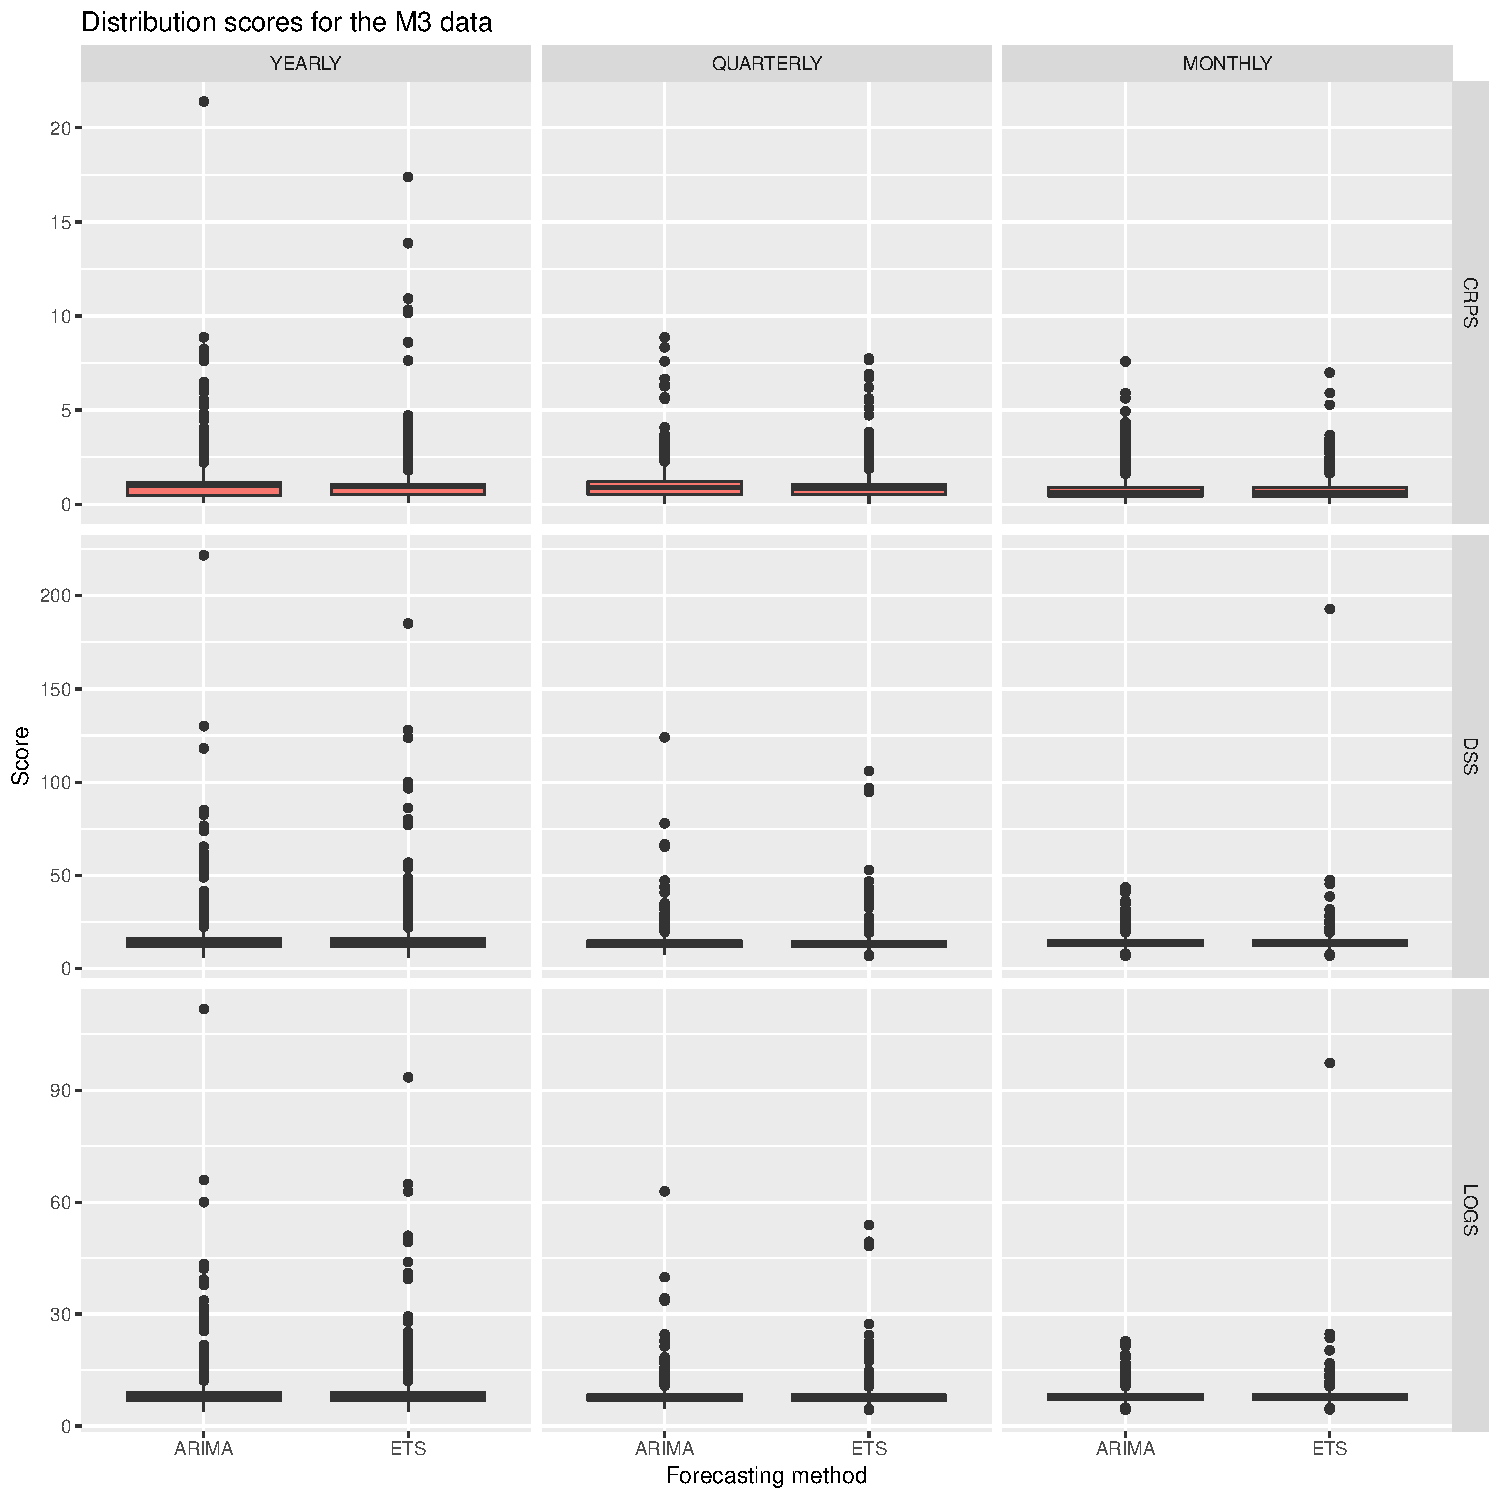
\includegraphics[width=1\linewidth]{thesis_files/figure-latex/boxplot-1}

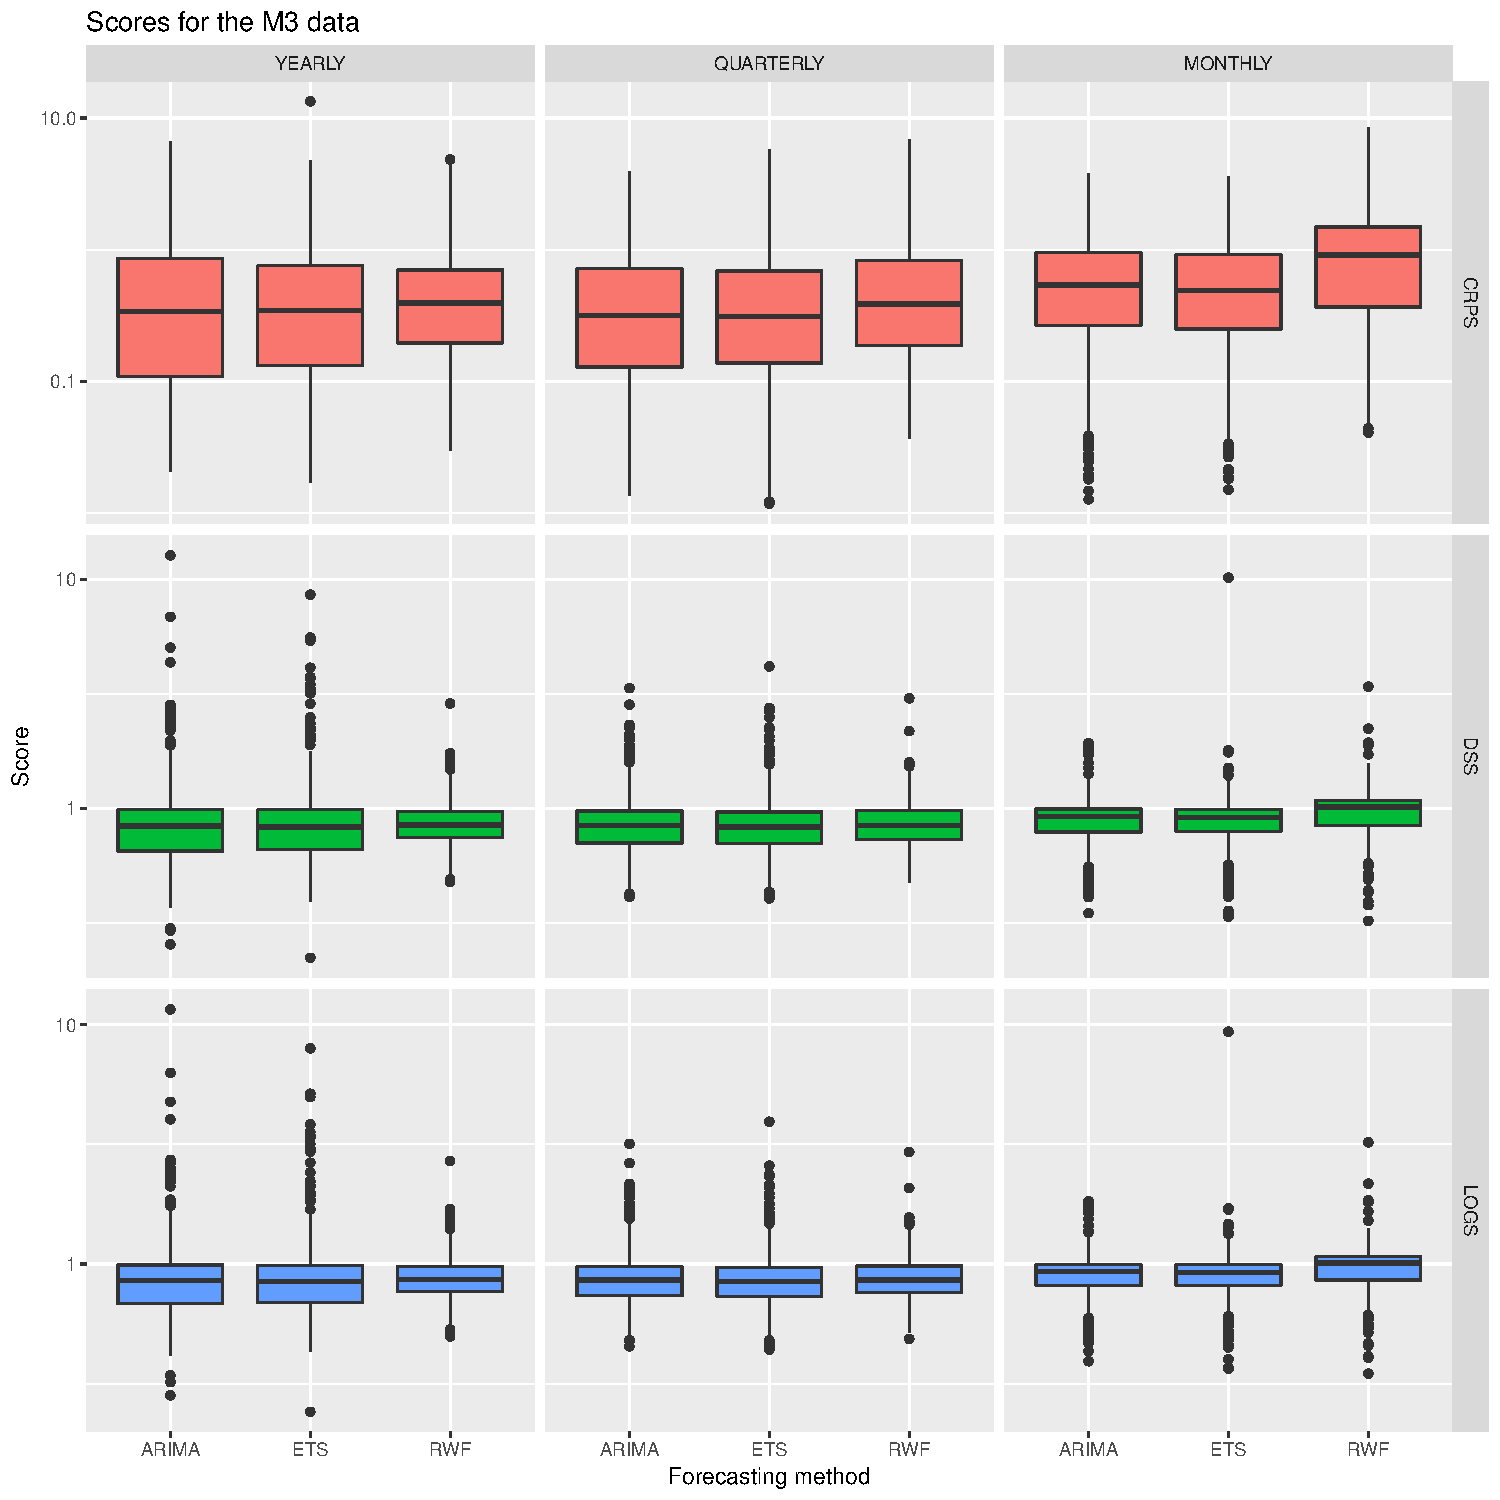
\includegraphics[width=1\linewidth]{thesis_files/figure-latex/boxplotlog-1}

Although it cannot be known from the above figure how many outliers are
generated base on the different forecast model by different scoring
rules, boxplots can show 5th, 25th, 50th, 75th and 95th percentiles of
central prediction interval width. The width of the obvious random walk
model is much narrower than that of other models, which means that its
sharpness is sharpest, and the calibration is more accurate, although
its mean value is not the lowest. Therefore, in the case of using M3
data sets, the quality of probability predictions derived from random
walk model is even higher. This also proves that using scoring rules can
simultaneously evaluate the sharpness and calibration of probabilistic
results.

\chapter{Conclusion}\label{conclusion}

In this report, we introduced what is the probabilistic forecasts, and
calibration and sharpness. It also introduced scoring rules. For the
three commonly used scoring rules, we show their original formulas and
form under Gaussian predictive distribution. In the section of the case
study, we first used two models to do probabilistic forecasts for the
ASX200 index, to evaluate the forecasts results by using scoring rules.
Then we learned how to use scoring rules to evaluate the outcome of
forecasts. In the second case study, we used the M3 datasets and used
multiple models to do probabilistic forecasts. We learned how the
scoring rules evaluated both the probabilities and the results of car
calibration and sharpness.

\chapter{References}\label{references}

\begin{itemize}
\item
  Edgar C. Merkle, Mark Steyvers (2013) Choosing a Strictly Proper
  Scoring Rule. \emph{Decision Analysis} 10(4):292-304.
\item
  Gneiting T, Balabdaoui F, Raftery AE. (2007). Probabilistic forecasts,
  calibration and sharpness. \emph{J. R. Stat. Soc. B} 67:243--68
\item
  Gneiting, T., \& Katzfuss, M. (2014). Probabilistic forecasting.
  \emph{Annual Review of Statistics and Its Application}, 1(1),
  125--151.
\item
  Gneiting T, Raftery AE. 2007. Strictly proper scoring rules,
  prediction, and estimation. \emph{J. Am. Stat. Assoc.} 102:359--378
\item
  Hersbach, H. (2000), ``Decomposition of the Continuous Ranked
  Probability Score for Ensemble Prediction Systems,'' \emph{Weather and
  Forecasting}, 15(5),559--570.
\item
  Hyndman, R. J. (2018). forecast: Forecasting functions for time series
  and linear models (R package version 8.3).
  \url{https://CRAN.R-project.org/package=forecast}
\item
  Hyndman, R. J., \& Athanasopoulos, G. (2018). Forecasting: principles
  and practice. 2nd ed., Melbourne, Australia: OTexts.
  \url{https://OTexts.org/fpp2/}
\item
  Hyndman, R. J.(2018).Data from the M-Competitions (R package version
  2.7). \url{https://CRAN.R-project.org/package=Mcomp}
\item
  Jordan. A., Krueger. F., Lerch. S. (2017). Scoring Rules for
  Parametric and Simulated Distribution Forecasts. (R package version
  0.9.4). \url{https://CRAN.R-project.org/package=scoringRules}
\item
  Matheson, J. E., and Winkler, R. L. (1976), ``Scoring Rules for
  Continuous Probability Distributions,'' \emph{Management Science}, 22,
  1087--1096.
\item
  Peirolo. R. (2010). Information gain as a score for probabilistic
  forecasts. \emph{Meteorological Applications} 03/2011, Vol.18(1),
  pp.9-17
\item
  Raftery, A. E. (2016). Use and communication of probabilistic
  forecasts. \emph{Statistical Analysis and Data Mining: The ASA Data
  Science Journal}, 9(6), 397--410.
\item
  Roulston, M. S., and Smith, L. A. (2002), ``Evaluating Probabilistic
  Forecasts Using Information Theory,'' \emph{Monthly Weather Review},
  130(6), 1653--1660.
\item
  Wuertz. D. (2017). Rmetrics - Autoregressive Conditional
  Heteroskedastic Modelling (R package version 3042.83).
  \url{https://CRAN.R-project.org/package=fGarch}
\item
  Wickham. H. (2017). Easily Install and Load the `Tidyverse'. (R
  package version 1.2.1).
  \url{https://CRAN.R-project.org/package=tidyverse}
\end{itemize}

\printbibliography[heading=bibintoc]



\end{document}
